\selectlanguage{english}%

\chapter{Descrição do Sistema} \label{capDescSis}
Sistemas controlados são constituídos essencialmente por uma ou mais plantas e por um dispositivo que implementará os algoritmos de controle aplicados à ela. O objeto neste trabalho de estudo é uma planta de Quatro-Tanques, descrita na seção a seguir, e o controlador utilizado é um CLP Rockwell 1756-L62, apresentado na seção homônima logo em seguida.

\section{Sistema de Quatro-Tanques}
Em 1999, Karl Henrick Johansson publicou o artigo "Theaching Multivariable Control Using the Quadruple-Tank System" \cite{johansson2}, onde são apresentadas as ideias do sistema de quatro-tanques estudado neste trabalho. Trata-se de um laboratório didático de processo multivariável capaz de demonstrar dinâmicas de zeros alocáveis em fases mínima e não-mínima. Além disso, ilustra claramente os problemas de controle MIMO (Multiples Inputs Multiples Outputs) com acoplamento e de sistemas não lineares.

Seu diagrama esquemático é apresentado na  \hyperref[figDesc4tank]{Figura \ref{figDesc4tank}} a seguir. Ele consiste em quatro tanques interconectados, um reservatório inferior, quatro válvulas esferas e duas bombas de corrente contínua.

\begin{figure}[H]
	\centering
	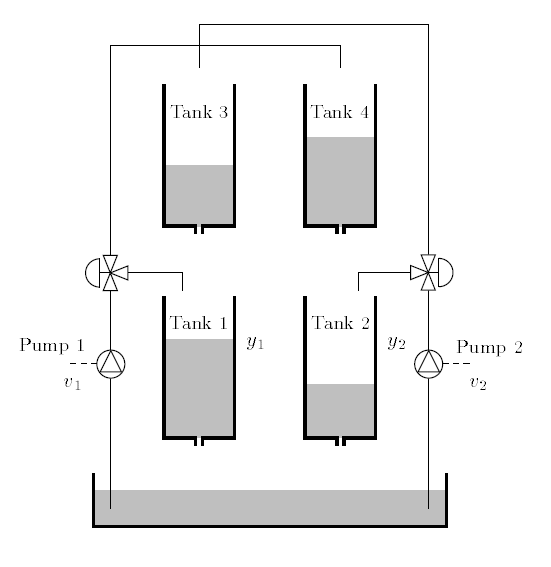
\includegraphics[width=0.5\textwidth]{img/4tank.png}
	\caption{\label{figDesc4tank}Diagrama esquemático do sistema de quatro tanques e planta didática.}
\end{figure}

As bombas impulsionam fluído por duas rotas: bomba 1 para os tanques 1 e 4, bomba 2 para os tanques 2 e 3.  As válvulas regulam a proporção direcionada entre os tanques inferiores e superiores de cada rota.

A \hyperref[imgPlanta]{Imagem \ref{imgPlanta}} a seguir apresenta a planta utilizada neste experimento, localizada no LARA (Laboratório de Automação e Robótica) - SG-11 (UnB) .

\begin{figure}[H]
	\centering
	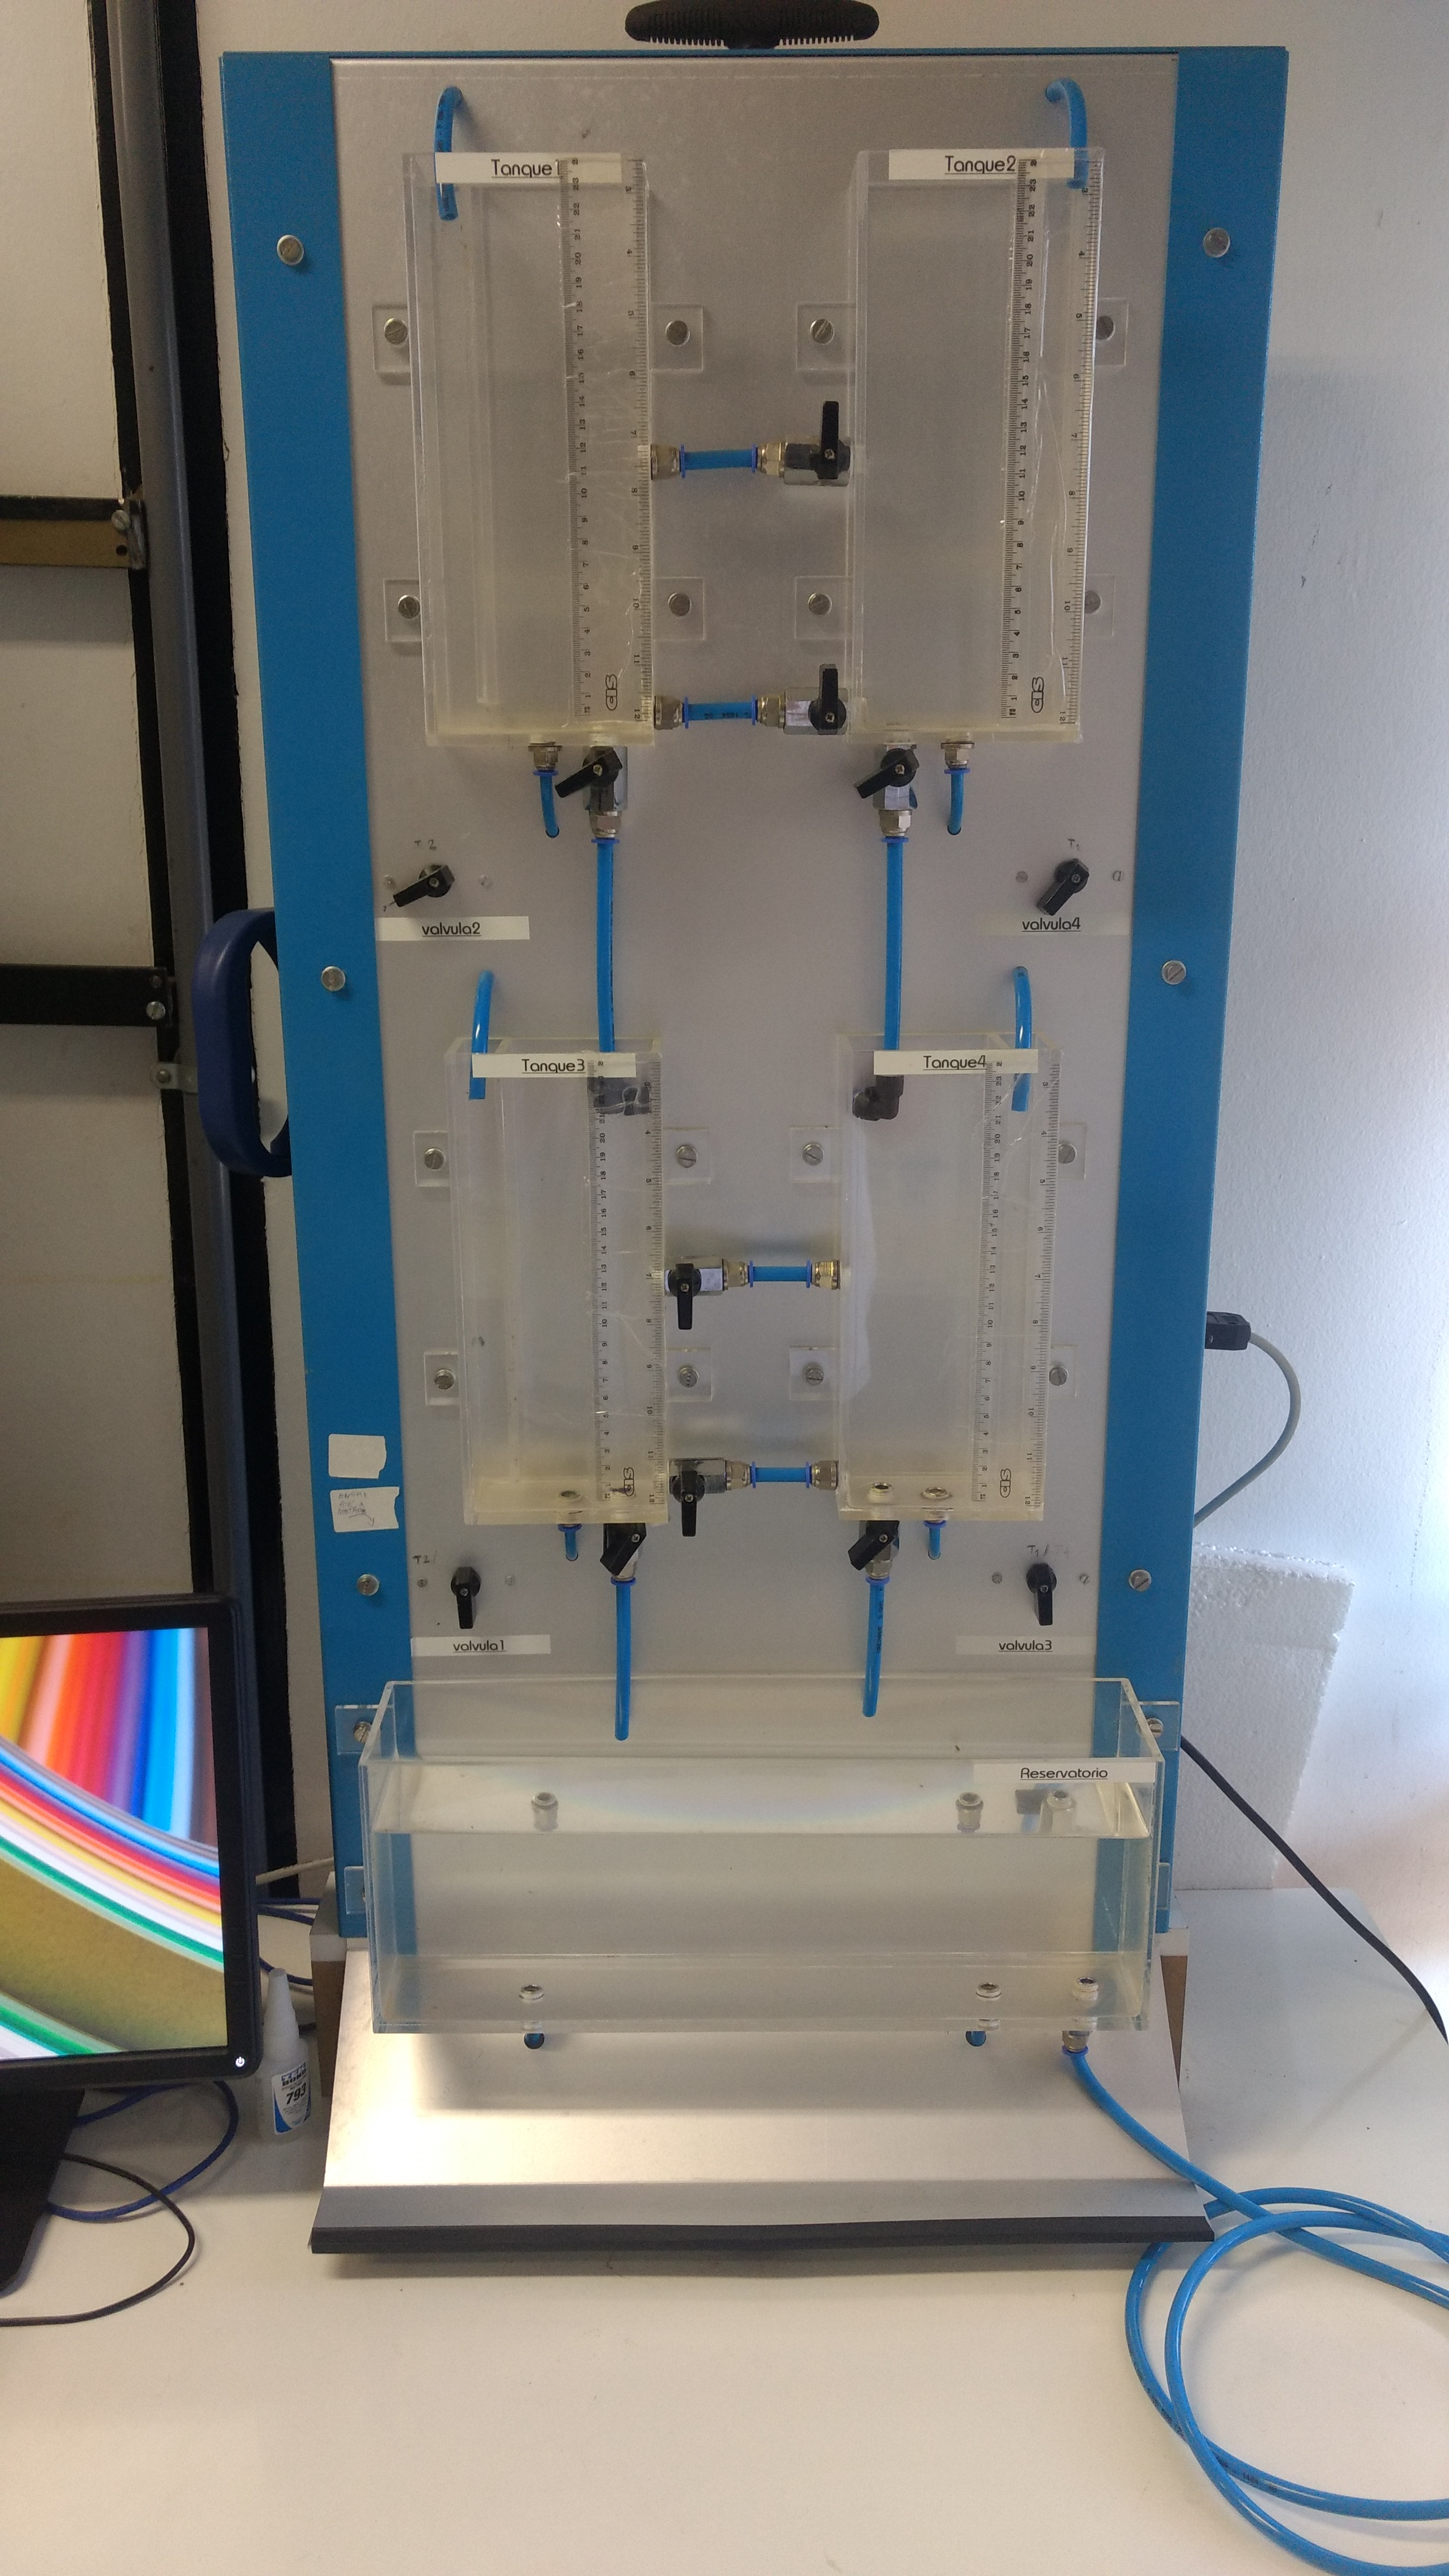
\includegraphics[width=0.4\textwidth]{img/tanqLara.jpg}
	\caption{\label{imgPlanta}Planta de Quatro-Tanques no LARA.}
\end{figure}

Suas dimensões aferidas são apresentadas na \jhhref{tabDescPlanta}{Tabela}, onde $A_{i}$ e $H_{i}$ representam a área da secção transversal da base do tanque e  o nível máximo do tanque $i$, $i = 1,2,3,4$.  $\gamma_{1}$ é a razão entre os fluxos para os tanques 1 e 4 e $\gamma_{2}$ é a razão entre os fluxos para os tanques 2 e 3. 

\begin{table}[!ht]
	\caption{Especificações Iniciais da Planta.}
	\label{tabDescPlanta}
	\small
	\centering
	\scalebox{1}{
			\begin{tabular}{|c|c|}
			\hline
			\multicolumn{2}{|c|}{Especificações Iniciais da Planta} \\
			\hline
			A1, A3 & 47,6 cm$^2$ \\ \hline
			A2, A4 & 47,6 cm$^2$\\ \hline
			H1, H2, H3, H4 & 24 cm\\ \hline
			g & 981 cm/s$^2$ \\ \hline
			$\gamma_1$ & 0.70 \\ \hline
			$\gamma_2$ & 0.60 \\ \hline
		\end{tabular}
	}
\end{table}

\section{CLP Rockwell 1756-L62}
Controladores Lógico Programáveis (CLP) são largamente utilizados para controle de processos e automação industrial atualmente. Trata-se de um equipamento eletrônico digital com hardware e software adaptados para as condições industriais. Utilizam uma memória programável para armazenar instruções de controle e conexões com diversos módulos para interface com processos externos, entrada e saída de dados, comunicação digital, entre diversas outras funções.

\subsection{Instalação}
Neste trabalho realizou-se a montagem de toda a estação de controle. Assim, escolheu-se primeiramente um local adequado para a disposição do painel de controle: próximo à planta e ao microcomputador ao qual se conecta, porém afastado de fiações elétricas ou locais úmidos. Outro cuidado deve de ser observado durante a instalação da fonte junto ao chassi, observando a compatibilidade com as tensões de entrada e saída do controlador. Seguiu-se fixação do painel no local escolhida, instalação do microcomputador à ser utilizado e instalação da fiação elétrica. Observa-se na Figura \ref{fig:mesa} o resultado instalado.

\begin{figure}[H]
	\centering
	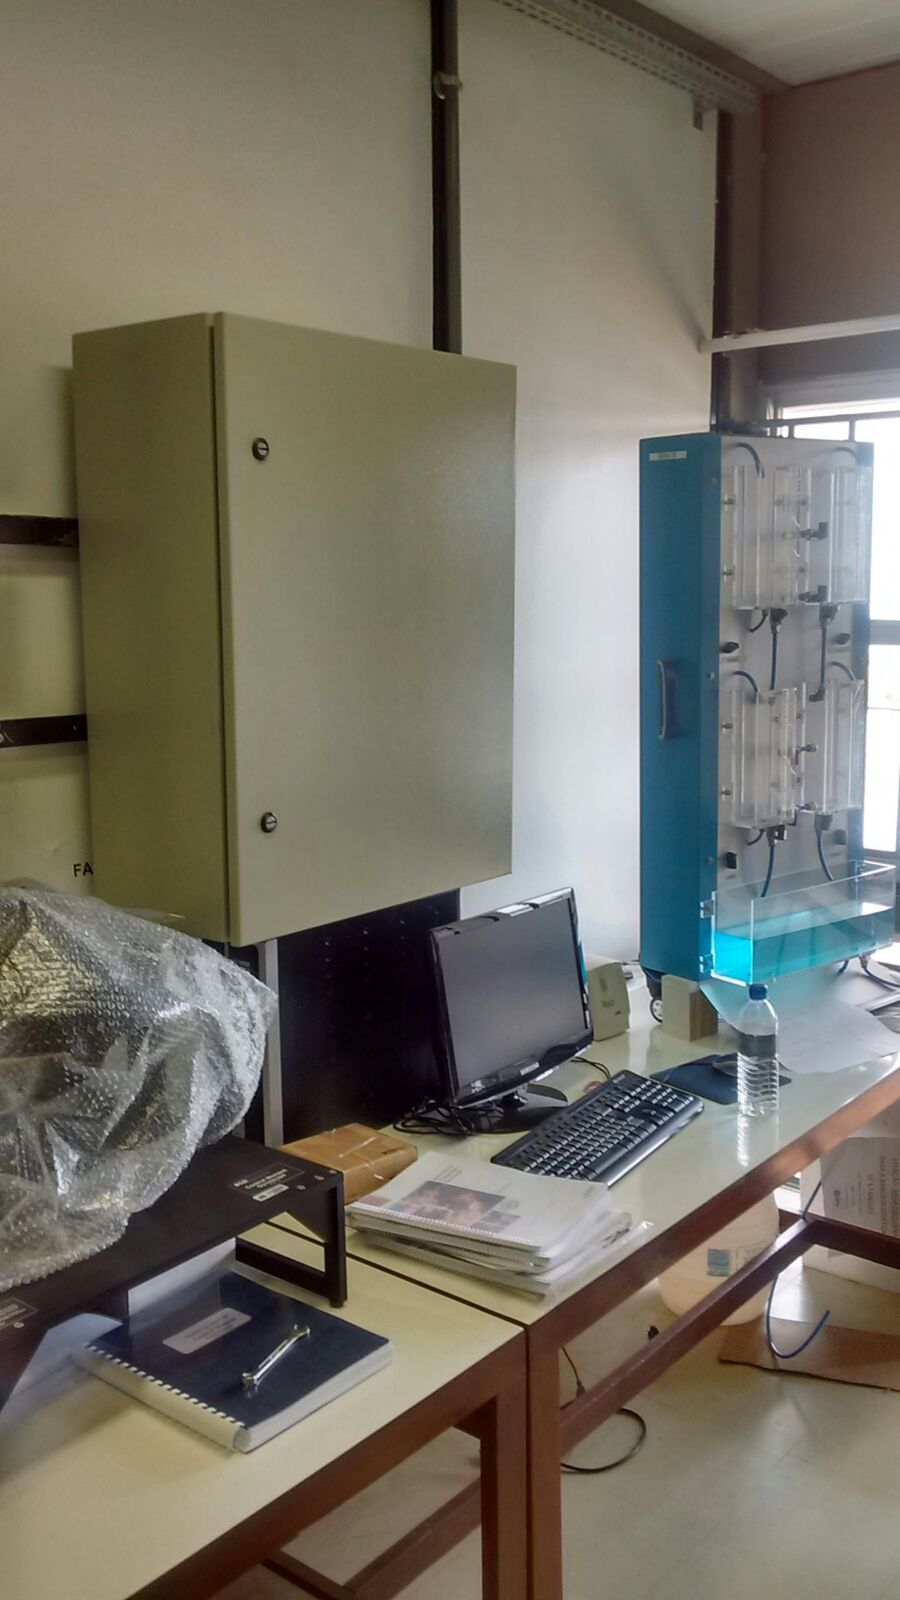
\includegraphics[height=10cm,keepaspectratio]{figs/mesa.jpg}
	\caption{Estação de trabalho.}
	\label{fig:mesa}
\end{figure}

A Figura \ref{fig:interior} a seguir ilustra o interior do painel, já com o chassi do controlador instalado e as trilhas utilizadas distribuídas no espaço restante para conexão dos bornes a serem utilizados no projeto.

\begin{figure}[H]
	\centering
	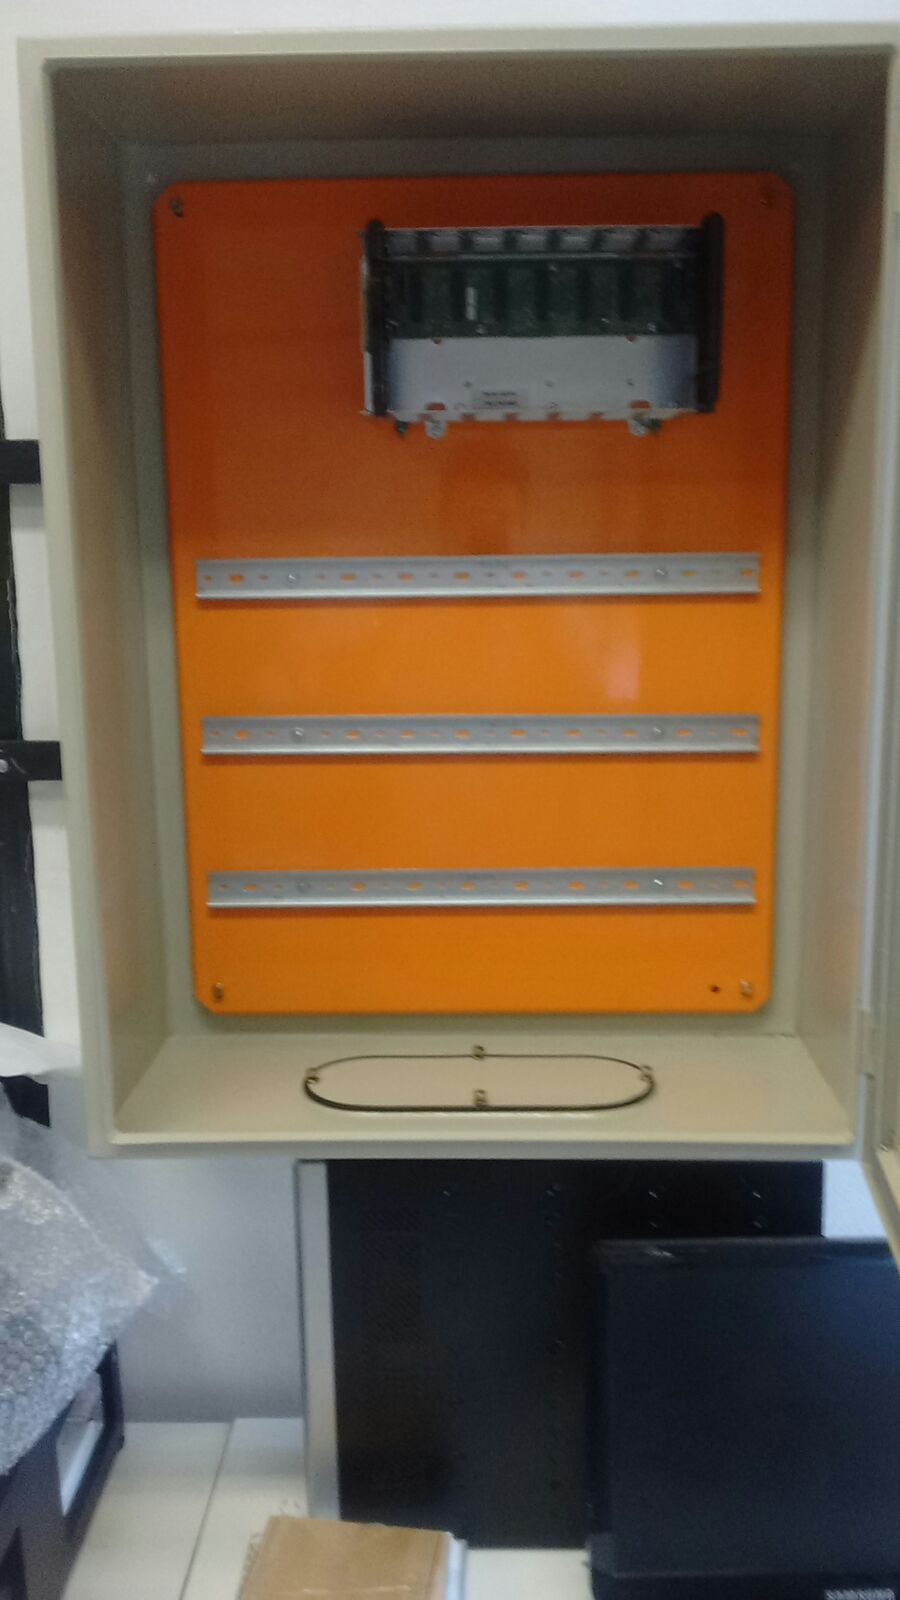
\includegraphics[height=10cm,keepaspectratio]{figs/interior.jpg}
	\caption{Interior do painel.}
	\label{fig:interior}
\end{figure}

Os módulos de entrada e saída foram instalados conforme a \hyperref[tab:modulos]{Tabela \ref{tab:modulos}} abaixo. 

\begin{table}[!ht]
	\caption{Módulos 1756 instalados.}
	\label{tab:modulos}
	\small
	\centering
	\scalebox{1}{
		\begin{tabular}{|c|c|c|}
			\hline
			Especificação & Descrição & Posição no chassi\\
			\hline
			1756-A7/B & Chassi & .\\
			\hline
			1756-L62 & Controlador & 0 \\
			\hline
			1756-ENBT/A & EtherNetIp & 1\\
			\hline
			1756-IF8/A & Entradas Analógicas & 2\\
			\hline
			1756-OF8/A & Saídas Analógicas & 3\\
			\hline
			1756-IB16/A & Entradas DC & 4 \\
			\hline
			1756-OB8I/A & Saídas DC & 5 \\
			\hline
		\end{tabular}
	}
\end{table}

Observa-se na Figura \ref{fig:modulos} a seguir a configuração instalada.

\begin{figure}[H]
	\centering
	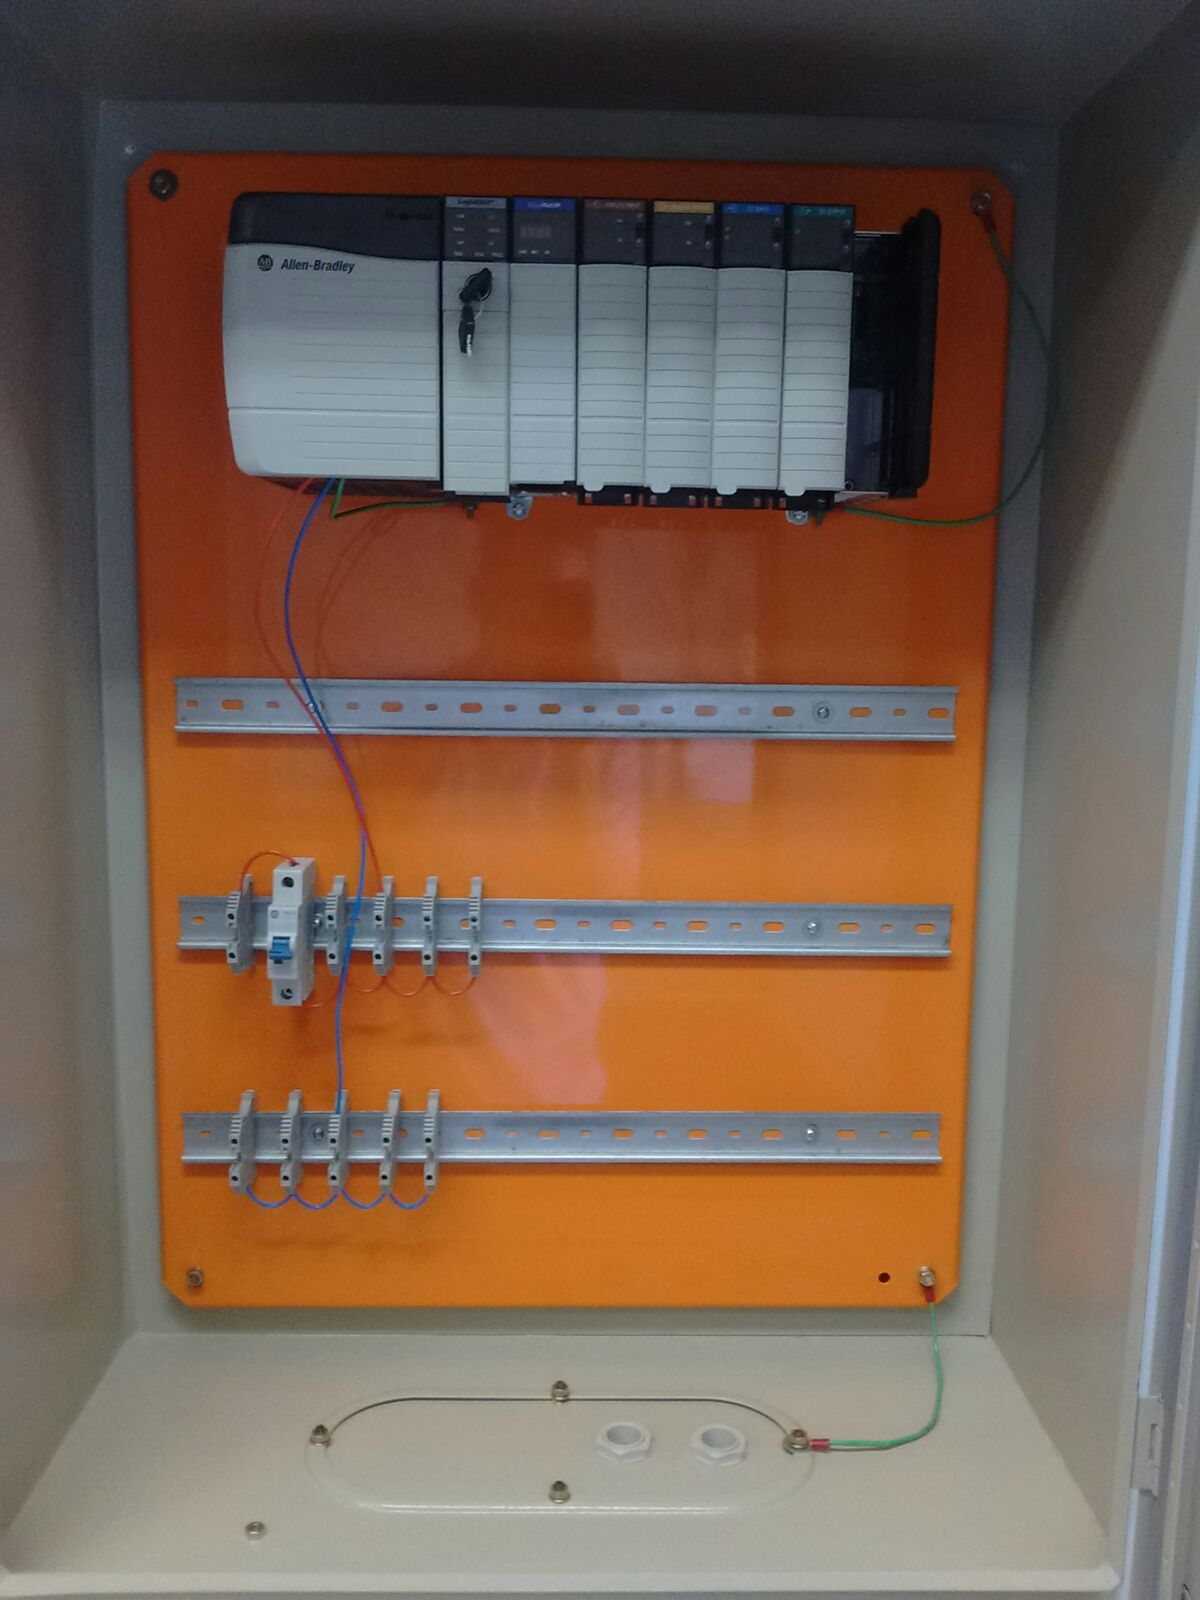
\includegraphics[height=10cm,keepaspectratio]{figs/modulos.jpg}
	\caption{Módulos do painel.}
	\label{fig:modulos}
\end{figure}

\subsection{Integração}
Seguiu-se a configuração dos módulos de comunicação com o CLP. Dois modos são disponíveis com os módulos utilizados: serial, realizada diretamente com o controlador, e Ethernet, através do módulo EtherNetIP. Ambas foram implementadas e testadas.

Para comunicação serial, basta configurar a entrada serial no computador a ser utilizado e em seguida configurar o controlador no software RSLinx \cite{rslinx}. Para utilizar a comunicação EtherNetIp é necessário antes configurar o módulo EhterNetIp \cite{ethernetmodule}. O software BOOTP/DHCP torna possível assinar um endereço IP para o módulo recém instalado. Para que a comunicação em uma rede EtherNetIp ocorra corretamente todos os dispositivos dela precisam possuir endereços IP seguindo o padrão definido pela máscara de sub-rede, neste caso, 255.255.255.0. Isso significa, basicamente, que os pontos comunicantes da rede devem possuir ids únicos apenas nos último octeto de seus endereços. A tabela a seguir apresenta os endereços utilizados, bem como a configuração padrão da rede.

\begin{table}[!ht]
	\caption{IPs dos dispositivos}
	\label{tabIPs}
	\small
	\centering
	\scalebox{1}{
		\begin{tabular}{|c|c|}
			\hline
			\textbf{Dispositivo} & \textbf{Endereço}\\
			\hline
			PC (RSLinx) & 192.168.2.1\\
			\hline
			1756-ENBT/A (CLP) & 192.168.2.22 \\
			\hline
			Geral & 192.168.2.xxx\\
			\hline
		\end{tabular}
	}
\end{table}

Um \textbf{importante} cuidado de segurança observado foi o aterramento de diversos elementos do equipamento. É conhecida sua capacidade de operação em condições adversas, mesmo assim, como precaução houve o cuidado de aterrar o chassi, a placa onde foi instalado e o painel exterior.

\section{RSLinx e RSLogix}
Os principais softwares utilizados para implementação do controlador são o RSLinx e o RSLogix. O primeiro é responsável por estabelecer a comunicação com o CLP Rockwell e sua ampla variedade de aplicativos e módulos. A \jhhref{imgRSLinx}{Figura} apresenta sua interface, onde é possível visualizar o controlador e os módulos instalados. A partir deste menu são acessíveis diversas funções de configuração e exibição das informações dos dispositivos.

\begin{figure}[H]
	\centering
	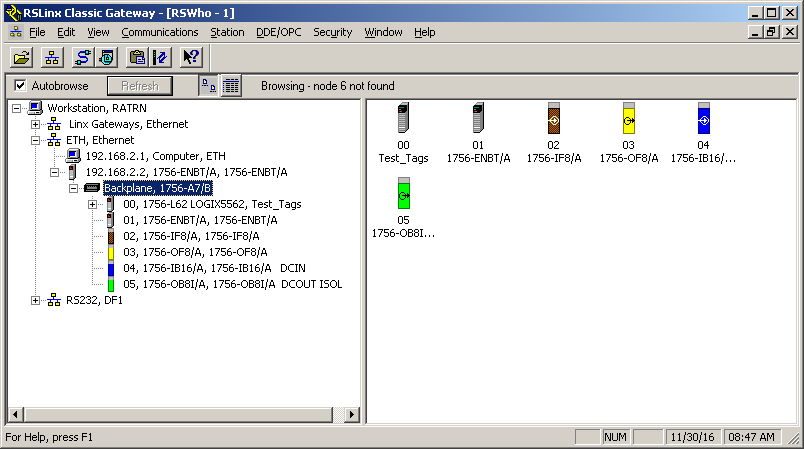
\includegraphics[height=5cm,keepaspectratio]{img/RSLinx.png}
	\caption{Interface do Software RSLinx.}
	\label{imgRSLinx}
\end{figure}

Já o RSLogix 5000 é o ambiente de desenvolvimento proprietário da Rockwell (Allen-Bradley). Neste trabalho, os controladores foram desenvolvidos no RSLogix e enviados (Download) para o CLP em conjunto com o RSLinx. As seções a seguir apresentam as linguagens de o desenvolvimento disponibilizadas pelo RSLogix, a saber linguagem Ladder, blocos de funções e texto estruturado.

\subsection{Linguagem Ladder} \label{subsec:ladder}
A linguagem Ladder é a pioneira dos CLPs por se tratar de uma evolução natural de diagramas elétricos, utilizados antes da chegada dos controladores digitais.  Seu ambiente de desenvolvimento utiliza o posicionamento de de símbolos e blocos para implementação da lógica de controle. 
O ambiente inicial é formado por duas linhas verticais, que representam nível lógico alto (à esquerda) e baixo(à direita) de um sistema. Entre essa linhas são desenhados ramais horizontais que representam representados os estados do CLP.

Uma forma de compreender essa linguagem seria como uma série de conexões de contatos e bobinas. Se for possível traçar um caminho da esquerda para direita, conectando-se à uma bobina de saída ao final, então o valor dessa bobina será verdadeiro. Trabalhando-se com controladores digitais, são criadas variáveis no programa que representam diretamente os valores presentes nos módulos de saída e entrada. Essas variáveis recebem o nome de TAGs. Assim, as variáveis de entradas são assinaladas à tags utilizadas como chaves e as variáveis de saídas à tags associadas às bobinas de saída. Percorrendo-se o caminho da esquerda para direita em um ramal, ao se chegar à uma chave, observa-se se o valor assinalado à ela é verdadeiro. Caso seja, continua-se o caminho até uma bobina de saída. Se está for alcançada, seu valor é setado para verdadeiro, consequentemente a saída associada a ela recebe a tensão associado à este nível lógico no controlador.

A Figura \ref{fig:ladder} à seguir ilustra um exemplo.

\begin{figure}[H]
	\centering
	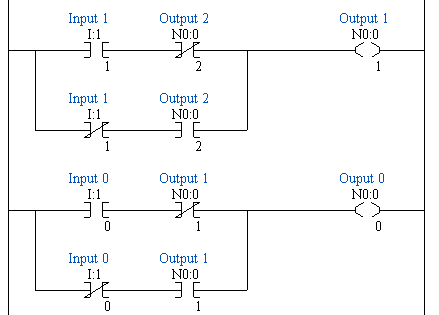
\includegraphics[height=5cm,keepaspectratio]{figs/ladder.png}
	\caption{Exemplo de Diagrama Ladder.}
	\label{fig:ladder}
\end{figure}

\subsection{Blocos Funcionais} \label{subsec:blocos}
Trata-se de outra linguagem de programação gráfica disponível aos CLPs Rockwell. É bastante semelhante à observada em vários outros softwares comuns ao meio acadêmico, como o MATLAB. Para sua utilização, assinala-se tags às entradas e saídas dos módulos já adicionados ao projeto. O desenvolvimento utiliza blocos de entradas e saídas associados à essas variáveis. Conexões entre os blocos, por meio de linhas representam passagem dos valores por esses fios. A lógica de controle é feita por meio de blocos de funções, estes possuem uma ou mais entradas e uma ou mais saídas. Os valores assinalados à suas saídas são determinados pelas funções às quais estão associados e que utilizam os valores de entrada como argumentos.

A Figura \ref{fig:blocos} à seguir ilustra um exemplo.

\begin{figure}[H]
	\centering
	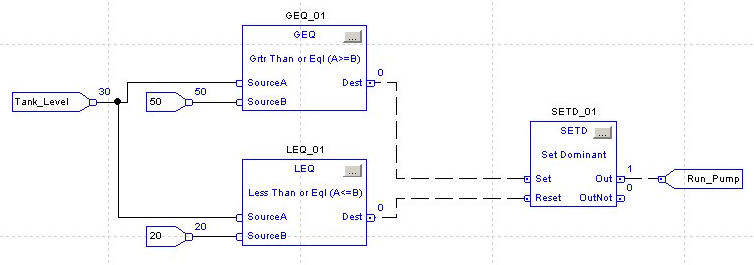
\includegraphics[height=5cm,keepaspectratio]{figs/blocos.png}
	\caption{Exemplo de diagrama de blocos.}
	\label{fig:blocos}
\end{figure}

Observa-se o caso do bloco GEQ\_01. Suas entradas são o nível do tanque (SourceA = Tank\_Level) e um valor constante (SourceB = 50). Sua saída (dest) será assinalada com nível lógico verdadeiro apenas quando $SourceA \geq SourceB$, ou seja, $Dest=1$ se $Tank\_Level \geq 50$, sendo $Dest = 0$ caso contrário.

\subsection{Texto Estruturado} \label{secTexEst} 
A linguagem texto estruturado é muito semelhante às linguagens estruturais C e Pascal. Como elas, é baseada no uso simples de comandos que são executados sequencialmente em seu desenvolvimento. Da mesma forma que as anteriores, esta linguagem utiliza Tags como variáveis e é a partir delas que se faz a leitura das entradas e definem-se as saídas. 

A \jhhref{imgTexEst}{Figura} à seguir ilustra um exemplo.

\begin{figure}[H]
	\centering
	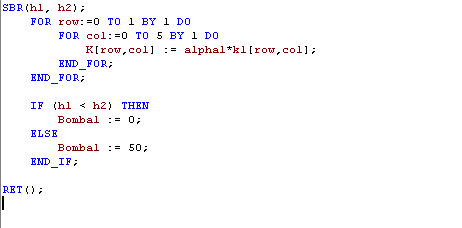
\includegraphics[height=5cm,keepaspectratio]{img/strText.png}
	\caption{Exemplo de Texto Estruturado.}
	\label{imgTexEst}
\end{figure}

%% TODO: Exemplo
\selectlanguage{brazil}%

